\chapter{Scientific Overview: Goals \& Strategy}
\minitoc
%\pg
%This section aims to provide a general overview of our scientific aims \& chosen strategy. [describe more]

\section{Science Goal}
\pg
So far, we have shown the technical work done on interferometric techniques as part of this PhD. In this section, we outline the application of this work, along with other modern tools, to the creation of large, deep and high-resolution surveys of the sky. While this approach is potentially extremely rewarding in terms of the science one can do with its resulting maps, it is also uniquely complicated.

\pg
Why, then, use this approach? One reason is the challenge itself. A high-resolution (matching HST resolution), wide-area (multiple degrees wide), high-quality\footnote{Reliably artefact-free, with known \& limited decorrelation, etc.} radio survey has \emph{never} been achieved at the time of writing. Many surveys of the radio sky exist, of course, but they tend to combine only two of those three qualities. FIRST \citepads[see][and references therein]{2015ApJ...801...26H}, for example, has achieved tremendous results with a $4''$ resolution, relatively low sensitivity, and no short baselines (thereby missing diffuse emission and extended structure) at $\sim$1.4 GHz. The VLASS \citepads[see][and references therein]{2013arXiv1312.4602H} will aim to go to a $2.5''$ resolution, medium sensitivity, and few short baselines - at frequencies ranging from 2 to 4 GHz. There exist many LOFAR HBA ($\sim$120-240 MHz) sky surveys \citepads[cf.]{2016MNRAS.460.2385W,2017A&A...598A.104S}, but they do not yet make use of international LOFAR, and are thus limited in resolution ($\sim 5''$).%Finally, there will of course be the SKA1-MID survey once the SKA is operational; this survey is expected to provide excellent resolution, sensitivity, and good $uv$-coverage, making it sensitive to diffuse emission as well as point sources.

\pg
In this context, a sky survey made using international LOFAR would be competitive until the SKA-MID survey (and considering it maps the Northern sky rather than the Southern sky, would arguably remain competitive even then). It would also allow LOFAR to fulfill the role of pathfinder in a very literal way, by providing datasets on which algorithms and imaging strategies could be tested before handling SKA data volumes in real-time.

\pg
Making a high-resolution full-sky survey using international LOFAR is thus arguably useful in and of itself in terms of interferometric techniques \& instrumentation. What then of its science value? The two most obvious advantages of a good large-sky survey are that they are complete (i.e. they are an accurate sample of the underlying source distribution, up to the survey's limiting flux)  while still giving information on rare outlier objects which may happen to lie in the field. This gives us access to a wealth of statistics from which to derive more robust estimations of population distributions. %Furthermore, depending on the quality of a given survey, it might even be able to provide such statistics simultaneously for various different fields of scientific interest.

\pg
Of course, LOFAR is already providing such catalogues - LOTSS \citepads[see][and references therein]{2017A&A...598A.104S}  is only the first of many to come. But these catalogues do not make use of the LOFAR international stations, and thus do not make full use of LOFAR's resolution ($5''$ resolution vs. $0.5''$).  This is so due to the technical challenges introduced by the use of international stations, which are due to decorrelation and an already limited signal-to-noise on those very short spatial frequencies.

\pg
What would they add to a LOFAR catalogue? A high-resolution sky survey has all the advantages listed above with more besides. For AGN science, for example, the higher resolution gives information on smaller scales, which is very relevant to study the turbulent processes in the lobes and the nearby intergalactic medium. We also know that there exist small AGNs: size therefore matters, and resolving these small AGNs (which tend to lie at larger redshifts, hence their smaller angular size) can give extremely salient information on AGN population distributions as a function of the age of the universe. Indeed, for AGN science, the LOFAR international baselines can be the difference between having absolutely no information on size distribution (no resolved AGN) and knowing everything about the AGN size distribution within a given extragalactic field. Finally, resolving sources is very relevant to spectral studies of AGN populations: we know very little about the physics of AGNs at low frequencies. Information on large populations of resolved sources (allowing us to separate compact structure from extended emission) is a prerequisite to begin the statistical work needed to understand these low-frequency AGN physics. As such, the international baselines can bridge a critical gap in the data available to peers studying AGN science.

\pg
AGN science is far from the only field which could benefit from the sub-arcsecond resolution that international LOFAR could provide. High-resolution imaging can be of tremendous interest to the study of star-forming galaxies: it could give insight into cosmic ray structure and access to spectral information. This is relevant because the entire star-forming history of galaxies is encoded in radio emission, but can only be accessed with sufficient spectral information and spatial resolution. A high-resolution survey, in particular, allows comparisons between optical and radio emission for known star-forming galaxies on a truly industrial scale, which would allow for the mapping of free-free absorption, supernova remnants, HII regions, etc...onto optical maps, and this for sources going up to high redshifts.

\pg
Of course, this does not run the full range of science cases which would benefit from high-resolution maps of large parts of the radio sky. Colleagues studying gravitational lensing would benefit greatly from large samples of lensed galaxies. Resolved extragalactic recombination lines (for bright objects) would doubtlessly interest peers studying galactic evolution. We expect these samples to be a natural byproduct of a large, high-resolution map of the radio sky: if they do not appear, that could indeed be a very interesting scientific result in and of itself.

\pg
More generally, high-resolution surveys provide high-resolution images of everyone's favourite objects and sources. It allows for better optical matching and identification, which is particularly relevant e.g. when needing to associate either a low-z or high-z sources to optical counterpart sources (in the case of the Extended Groth Strip, for example, using the international stations means matching the Hubble Space Telescope's resolution). They are thus a strong contribution to multi-wavelength datasets. It also improves the image's sensitivity to compact sources embedded in diffuse emission: if the source is better-resolved, then the emission associated with compact sources is more easily separated from emission emitted by its surroundings. This can be of tremendous help in image interpretation. Finally, actually resolving objects allows us to have better morphological classification for compact objects, which can be extremely useful e.g. when interested in AGN populations vs star-forming galaxy populations.




\section{3C295 and the Extended Groth Strip}

\pg
In this section, we briefly describe previous observations of the Extended Groth Strip (EGS), an extragalactic field with a rich multi-wavelength coverage described in Table \ref{table.EGS.observation}. It has been long observed as part of the All-Wavelength Extended Groth Strip International Survey collaboration (AEGIS, \citetads{2007ApJ...660L...1D}), which later became part of the CANDELS collaboration (\citetads{2011ApJS..197...35G}). The field is centred at $\alpha=14^h17^m,\delta=+52\deg 30'$, placing it between the tail of Ursa Major and Draco. Its size is $0.7'\times 0.1'$. It has notably been the subject of very deep Hubble Space Telescope observations, which the international LOFAR could attempt to match. 

\begin{table}[h!]
\begin{tabular}{cccc}
Telescope    & Band    & Resolution  & Area \\\hline
Chandra      & X-ray   & $0.5''-6.0''$ & $17'\times 120'$ \\
GALEX        & UV      & $5.5''      $ & 1.25$^\text{o}$ diameter \\
HST/ACS      & Optical & $0.1''      $ & $10' \times 67'$\\
HST/NICMOS   & Optical & $0.35''     $ & 0.0128 deg$^2$\\
Megacam      & Optical & $1.0''      $ & 1 deg$^2$\\
IRAC         & IR      & $2.0''      $ & $10' \times 120'$ \\
Spitzer      & IR      & $5.9''-19'' $ & $10'\times 90'$\\
VLA          & Radio   & $1.2''-4.2''$ & $30' \times 80'$
\end{tabular}
\caption{\label{table.EGS.observation}Table recapitulating the multi-wavelength coverage of the Extended Groth Strip, with observations performed as part of the AEGIS (later, CANDELS) collaborations.}
\end{table}

\pg
3C295 is a 3C\footnote{Third Cambridge Catalogue of Radio Sources, a 1959 survey of of the Northern radio sky} source, and thus one of the brighter sources in the Northern radio sky. It lies less than a degree away from the centre of the Extended Groth Strip, which has two important consequences: first, that it can potentially be used as a calibrator source for LOFAR; second, that unless well-modeled and subtracted at the observing instrument's maximum resolution, its sidelobes will pollute the EGS such that very little scientifically useful information might be recovered from a given observation.

\pg
The first step towards acquiring a deep, high-resolution image of the Extended Groth Strip therefore consists of creating a good, high-resolution model of 3C295 at LOFAR frequencies. Creating this model is one of the key results of this thesis. Starting from a high-resolution VLA model of 3C295, subbands selected across the LOFAR bandwidth are self-calibrated in iteratively greater numbers until a given noise threshold is reached. The flux scale is then boot-strapped based on the results of \citet{arse}. This ensures that 3C295 will be adequately subtracted from all corrected visibilities - including international baselines - and thus that images made using these visibilities will not be polluted by sidelobes from 3C295. 
The work done towards this goal is shown in \cref{section.3c295}. %, and its result - a high-resolution spectral model of 3C295 - is shown below.
%
%\pg
%\textcolor{red}{show key result here}

\section{Imaging the Full Primary Beam}
\pg
After creating a high-resolution model of 3C295 to calibrate the international stations, we must create a low-resolution model of all the sources in the primary beam to both improve final calibration quality and subtract sources outside of the Extended Groth Strip when creating the final high-resolution images.

\pg
Initial direction-independent calibration is done using the same pipeline as for the Lofar Two-metre Sky Survey \citepads[LOTSS,][]{2017A&A...598A.104S}. The killMS-DDF facet-based pipeline \citepads[cf]{2015MNRAS.449.2668S,2016ApJS..223....2V,2017arXiv171202078T} is then used to perform direction-dependent calibration for the entire LOFAR primary beam. This allows us to reach a noise threshold of $\sim$233$\mu$Jy.

\begin{figure}[h!]
\centering
\includegraphics[width=0.95\textwidth]{images/{lofar.widefield}.png}
\caption{\label{plot.EGS.lofar.widefield} Full direction-dependent calibrated image of the LOFAR primary beam, centred on the EGS. Image made without international stations.}
\end{figure}

\pg
This work, and its results, are shown in \cref{section.EGS.lowres}. Note that the AEGIS observations summarised in \cref{table.EGS.observation} do not cover the full LOFAR primary beam. The sources observed at low resolution are therefore matched with Sloan Digital Sky Survey (SDSS, \citetads{2000AJ....120.1579Y}) images. Overlays are shown to highlight the wealth of interesting sources, and their optical counterparts, which can be picked up as a byproduct of producing high-resolution maps of the radio sky. We select 12 particularly interesting sources and show the results of source matching for these candidates. Overlays of the same SDSS images with NVSS (NRAO VLA Sky Survey, \citetads{1998AJ....115.1693C}) postage stamps are also shown for comparison. Many of the chosen sources do not lie within the Extended Groth Strip, and are therefore only imaged at low resolution, but follow-up images and observations could be made should the need arise.

\section{Test Decorrelation}
\pg
Before launching the EGS imaging run using all calibrated datasets, we measure the impact of direction-dependent effects on known sources in the field. Two direction-dependent effects are expected to dominate: decorrelation and differential gains. The first is modeled by the imager used, whereas the second is a function of the gain variability as a function of distance from the calibrator. Seven calibrator sources, lying at various distances and directions from the calibrator source, are examined. They are summarised in \cref{table.LOBOS.sources}, which is reproduced below.

\begin{table}[h!]
\begin{tabular}{ccccc}
\# & RA [hms]    & Dec [dms]   & Dist. from EGS [deg.] & Dist. from 3C295 [deg.] \\\hline
1  & 14:30:18.72 & 52:17:29.80 & 2.041                         & 2.904 \\
2  & 14:19:44.44 & 54:23:04.58 & 1.928                         & 2.517 \\ 
3  & 14:21:20.05 & 53:03:46.00 & 0.864                         & 1.743 \\
4  & 14:21:09.41 & 51:22:32.46 & 1.294                         & 1.728 \\
5  & 14:11:50.32 & 52:49:02.66 & 0.844                         & 0.619 \\
6  & 14:11:20.23 & 52:12:04.30 & 0.915                         & 0.000 \\
7  & 14:08:07.00 & 52:55:11.36 & 1.409                         & 0.869 \\
8  & 14:08:09.76 & 52:44:46.56 & 1.354                         & 0.680 \\
\end{tabular}
\caption{\label{table.LOBOS.sources1}Table recapitulating the positions of all 8 chosen calibrator sources, along with their distance from the observation phase centre (EGS phase centre) and calibrator phase centre (3C295), respectively.}
\end{table}
%\begin{figure}[h!]
%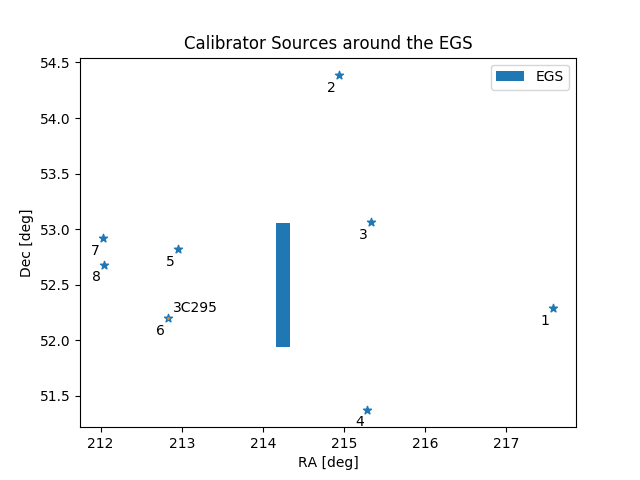
\includegraphics[width=0.8\linewidth]{images/EGS_LOBOS_scatterplot}
%\caption{Position of the calibrator sources around the EGS. Note that this is not projected properly onto the celestial sphere.}
%\label{bootes-coverage-image}
%\end{figure}

\pg
If directional gains are measured to have little or no impact, then direction-dependent calibration of the international stations will not be required. This is the ideal scenario, as it does not require the use of fringe fitting \citepads{1984ARA&A..22...97P}. If they are measured to have a significant impact, then direction-dependent calibration will be required for international LOFAR. We expect the angular scale of differential gain evolution to be of the order of a degree, and so most of the EGS should be relatively unaffected.


\section{Imaging the EGS with LOFAR international stations}

\subsection{Science Goals}

\pg
if decorrelation is merciful, proceed to patchwise imaging of EGS by using the results from the sections above (DI calibration using 3c295 model, followed by subtraction of all sources seen at low-res except within the patch we want to image; image, change patch; repeat until all EGS imaged)

\newpage